\section{Metolodgía de trabajo}

Nursoft se ha desenvuelto a lo largo de su vida en más de 20 proyectos de desarrollo de software. 
Los rubros de cada proyecto se extienden desde la minería, pasando por \textit{retail}, industria agropecuaria, 
mercado inmobiliario, \textit{e-learning} hasta en tele-medicina. 

Una mayoría importante de los proyectos caen en lo que es
\textbf{desarrollo de software clásico}, y el resto son entendidos como \textbf{consultorías}:
estos son proyectos donde el cliente está interesado inicialmente en conocer la factibilidad,
tanto comercial como técnica, de alguna propuesta o solución tecnológica generada por terceros o ellos mismos.

El primer grupo de proyectos se puede ceñir a una estructura informal de procesos como la siguiente:

\begin{itemize}
  \item Cliente presenta su necesidad/problema
  \item Nursoft indaga el estado actual del cliente para contextualizar la necesidad/problema
  \item Nursoft propone una solución
  \item Se realiza la planificación (junto con diseños necesarios)
  \item Se realiza la implementación
  \item Se realizan entregas periódicas
\end{itemize}

Por otro lado, las consultorías se ciñen a la siguiente estructura de procesos:

\begin{itemize}
  \item Cliente presenta su necesidad/problema junto con su propuesta
  \item Nursoft indaga el estado actual del cliente para contextualizar la necesidad/problema y la propuesta entregada
  \item Nursoft propone una contra-propuesta o modifica la propuesta entregada
  \item Nursoft valida la factibilidad comercial
  \item Nursoft valida la factibilidad técnica
\end{itemize}

\newpage 

La naturaleza diversa de los proyectos, tanto en dominio de conocimiento como en los procesos envueltos para 
llevarlos a cabo exitosamente, promueven una metodología flexible, pero bien definida; modularizada
y capaz de adaptarse a las diferencias de cada proyecto. Esta metodología se presenta en la Figura \ref{fig:procesos}.


\begin{figure}[h]
    \centering
    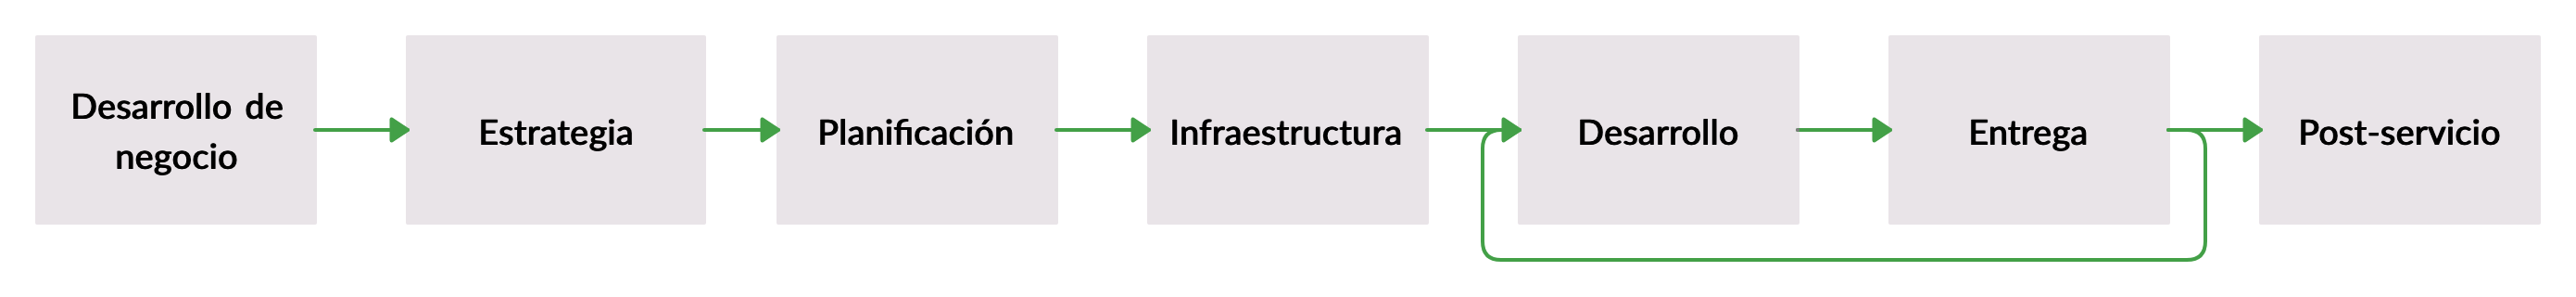
\includegraphics[scale=0.15]{procesos}
    \caption{Diagrama de macroprocesos para proyecto de desarrollo de software}
    \label{fig:procesos}
\end{figure}

La estructura general es adaptable a todo tipo de proyecto que Nursoft ofrezca, a modo de ejemplo, la Figura \ref{fig:consultoria}
ejemplifica la metodología de trabajo para un proyecto de consultoría.

\begin{figure}[h]
    \centering
    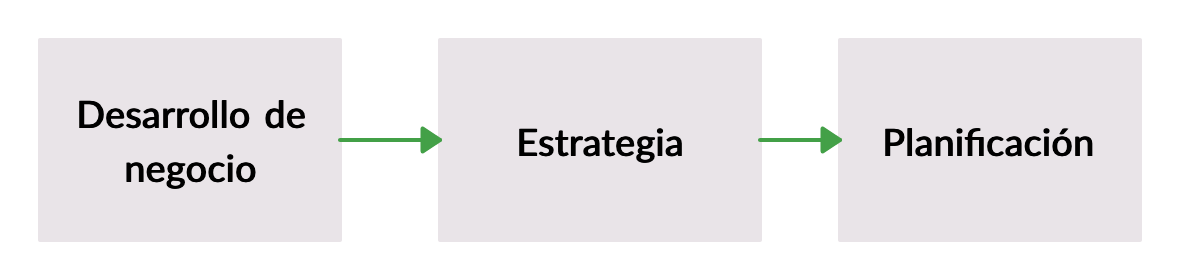
\includegraphics[scale=0.15]{consultoria}
    \caption{Diagrama de macroprocesos para proyecto de consultoría}
    \label{fig:consultoria}
\end{figure}


A continuación, se contextualiza brevemente cada macroproceso.

\subsection{Desarrollo de negocio}

El desarrollo de negocio en Nursoft, es el proceso que en una empresa más tradicional se llamaría Venta.
La diferencia es sútil, puesto que Nursoft deja en claro que no vende software como un ítem, vende el desarrollo
de software como una experiencia exclusiva y un servicio altamente flexible y con atención extra al detalle. 
El desarrollo de un negocio implica necesariamente crear una instancia donde ambas partes busquen la mejor parte de
trabajar en conjunto.

En esta etapa se nivelan las expectativas de ambas partes. También se mide la
compatibilidad del cliente con la empresa, con un potencial escenario donde el proyecto no sea aceptado por Nursoft.

Los puntos de mayor importancia de este macroproceso son el levantamiento de necesidades (una versión preliminar de requerimientos),
la creación de la propuesta económica y tecnológica y la firma de contrato. Para el caso de consultorías,
el levantamiento de necesidades se posterga para un macroproceso posterior.

\subsection{Estrategia}

Si la fase de \textbf{Desarrollo de negocios} fue éxitosa, este proceso sigue en el ciclo de vida de un proyecto.

En Nursoft se entiende estrategia como la define Chandler\cite{chandler_1962}:

\begin{displayquote}
Estrategia es la determinación de las metas y objetivos de largo plazo de la empresa,
y la adopción de caminos de acción y de asignación de recursos para alcanzar dichas metas…
\end{displayquote}

En este macroproceso se trabajan cuatro pilares en pos de una visión macro del proyecto:

\begin{itemize}
    \item El cliente
    \item El negocio del cliente
    \item Los usuarios
    \item El software
\end{itemize}

En otras palabras, se define formalmente cuál es el problema o la necesidad del cliente, contextualizada
a elementos internos y externos.

En términos prácticos, en esta etapa participa tanto el departamento comercial como el departamento de diseño
y experiencia de usuario (UX). El primer departamento trabaja para definir directrices de planificación
estratégica a la empresa del cliente (si así lo lo requiera), realizar estudios financieros
para analizar los impactos en el negocio que tendrá el proyecto. 
Al mismo tiempo, el departamento de UX investiga bajo que tipo de interacciones las hipótesis
comerciales del cliente son válidas. Para esto se utilizan diversas metodologías de
investigación del usuario: focus groups, entrevistas y encuestas. 

Este proceso termina con un entregable: la creación de la protopersona\footnotemark[7],
resultado que tendrá un rol protagónico en el siguiente macroproceso.

\footnotetext[7]{La proto-persona es el resultado de contrastar las visiones y expectativas
de un usuario ideal por parte de los \textit{stakeholders} con las expectativas de potenciales
usuarios reales que coincidan con ciertos criterios definidos de los \textit{stakeholders},
por ejemplo rango etario o nivel socioeconómico.}

\subsection{Planificación}

La \textbf{planificación} es el proceso en el cuál se responde qué solución se dará al problema definido en la \textbf{estrategia}.

Esta solución se propone, se investiga y se argumenta tanto desde lo técnico hasta de lo visual.

En su defecto, la planificación cuenta con cuatro fases:
\begin{itemize}
    \item \textbf{Propuesta de solución inicial}
    En la primera propuesta se realizan las mitigaciones técnicas necesarias, y según se necesite se 
    desarrollan los Diagramas de procesos
    \item \textbf{Desarrollo de marca} En donde Diseño realiza benchmarking e investigación
    de referentes, el \textit{naming}, la paleta de colores y tipografía y
    finalmente la creación de marca. Esta etapa es opcional, siempre se le sugiere al cliente y
    sólo se realiza bajo su mandato.
    \item \textbf{Diseño y experiencia de usuario}
    En donde aparecen los entregables más importantes para la posterior etapa de desarrollo. 
    Diseño genera el flujo de navegación, \textit{wireframes}\footnotemark[8] preliminares y el \textit{basic design system}\footnotemark[9].
    Estos son validados a través de pruebas de usabilidad con usuarios \textit{target}.
    El entregable final de esta etapa es un prototipo no funcinal hacia el cliente.
    \item \textbf{Propuesta de solucion técnica}
    En este último paso, los requerimientos son transformados en Historias de usuarios. Las historias se estiman utilizando la metodología de \textit{Planning Poker}\footnotemark[10].
    Utilizando como insumos los entregables de la propuesta inicial, se construye y presenta la propuesta de Arquitectura.
\end{itemize}

\footnotetext[8]{Un \textit{wireframe} es una esquemática o guía visual que muestra el esqueleto de una estructura.\cite{brown_2011}}
\footnotetext[9]{Un \textit{basic design system} es la única fuente de verdad que agrupa todos los elementos que permitirán al equipo identificar e implementar un producto, a nivel visual.\cite{kholmatova_2017}}
\footnotetext[10]{\textit{Planning Poker} es una técnica lúdica basada en consenso para estimar esfuerzo necesario para implementar una funcionalidad en desarrollo de software\cite{cohn_2012}}

\subsection{Infraestructura}

El proceso de Infraestructura es uno de los procesos más cortos de todo el flujo de desarrollo de un proyecto de software en Nursoft.
Sus entregables y responsabilidades son casi totalmente internos.

En este proceso se levanta la infraestructura tecnológica necesaria para el desarrollo del proyecto y la mantención del mismo.
Tomando como insumo la propuesta aceptada de Arquitectura, el equipo de Operaciones configura los servicios que serán utilizados
a través de plantillas automáticas. También se configuran los procesos automatizados de integración y despliegue continuo (\textit{CI} y \textit{CD}, respectivamente).

Finalmente, se configura el entorno de \textit{staging}, una versión de prueba de la plataforma final, utilizada para los subprocesos de \textit{Quality Assurance}\footnotemark[11]
y de revisión de Diseño.


\subsection{Desarrollo}

El proceso de desarrollo en Nursoft es un proceso iterativo, siguiendo una versión propia y modificada de \textit{SCRUM}.

La unidad mínima de trabajo en este proceso es el \textit{sprint}: es un período donde se trabaja en pos
de un objetivo de negocio claro. En este período el equipo completa una serie de funcionalidades acordadas al comienzo
del \textit{sprint} y relacionadas al objetivo.

La definición del objetivo generalmente quedo a criterio del equipo y su \textit{Project Manager}, pero una regla
fundamental es que cada \textit{sprint} debe generar valor para el cliente y/o el usuario.

Cada sprint se divide en tres etapas, como se muestra en la Figura \ref{fig:sprint}

\begin{figure}[h]
  \centering
  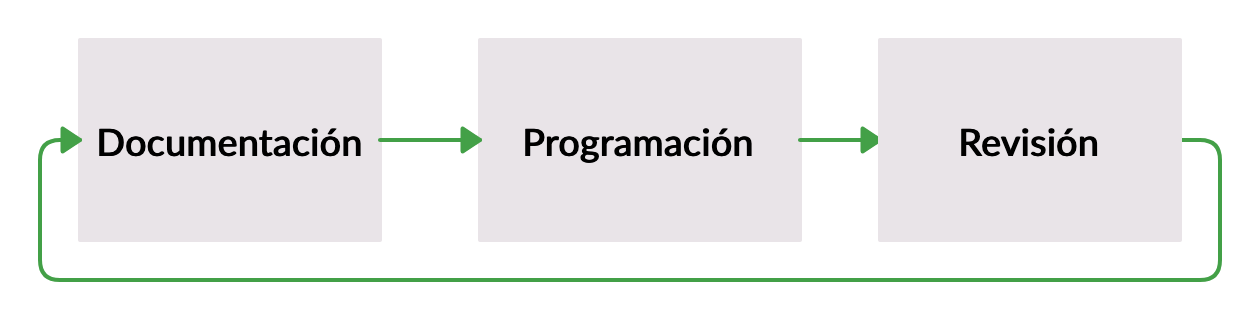
\includegraphics[scale=0.25]{sprint}
  \caption{Etapas de un sprint}
  \label{fig:sprint}
\end{figure}

\footnotetext[11]{\textit{Quality Assurance} es un término que engloba manera de prevenir defectos o fallas en un producto,
con el enfoque en entregar confianza de que los requerimientos serán cumplidos.\cite{iso_2005}}

\begin{itemize}
  \item \textbf{Documentación}
  Cómo se mencionó anteriormente, al comienzo de cada \textit{sprint} se define el objetivo de negocio, y con éste,
  las funcionalidades a implementar. Se discute y actualiza o completa la documentación de las
  historias de usuario correspondientes. 
  
  ¿Por qué revisitar la documentación en cada sprint si ya se definieron al final de la Planificación?

  Es común en la experiencia de Nursoft vivir de primera fuente uno de los fundamentos de la metodología ágil en
  cada \textit{sprint} mencionado en el capítulo anterior: 
  
  \begin{displayquote}
    Énfasis en software que funcione sobre una documentación amplia
  \end{displayquote}

  Esto es particularmente cierto para proyectos de desarrollo de software a medida.
  La documentación inicial fue útil para entender el alcance preliminar de la funcionalidad
  (además de cómo la arquitectura facilita su ejecución), pero a medida que el proyecto avanza,
  el cliente mismo va mejorando su conocimiento del contexto para cada funcionalidad, y al mismo tiempo refina
  sus expectativas de éste: plazos, integraciones, prioridad, etc. Por eso es relevante este subproceso de documentación
  al comienzo de cada \textit{sprint}: permite afinar al conocimiento disponible de todos los \textit{stakeholders} para la funcionalidad.

  \item \textbf{Programacion}
  Puntos relevantes para este subproceso son:
  \begin{itemize}
    \item La gestion del código en todos los equipos se hace a través de una versión modificada de \textit{Gitflow},
    un flujo de trabajo colaborativo para software de herramientas de control de versiones, como Git.
    \item El entregable de este subproceso es hacer el despliegue del código al ambiente de \textit{staging}.
    \item En la gran mayoría de los casos, el desarrollo de funcionalidades implica la generación de pruebas para este mismo.
    Particularmente, la mayoría de los equipos siguen el proceso de \textit{Test Driven Development} o \textbf{TDD}.
  \end{itemize}

  \item \textbf{Revisión}
  
  El proceso de revisión se constituye de dos tipos de revisiones: la manual y la automatizada.

  La \textbf{revisión automatizada} se realiza de manera continua durante el subproceso de programación, a través del proceso de Integración continua.
  Con cada sección de código enviada al repositorio central, se gatillan las pruebas automatizadas generadas en TDD. Si y sólo si las
  pruebas pasan, la sección de código enviada se mezcla con el repositorio.

  La \textbf{revision manual} cuenta con tres fases: \textit{code review}, revisiones de QA y revisión de diseño. Las revisiones de QA
  se ejecutan cuando las funcionalidades fueron completadas, y se llevan a cabo en el ambiente de \textit{staging}. 
  Su principal aporte es verificar una calidad mínima de la funcionalidad. Se realizan a través de un conjunto de casos de prueba o
  escenarios de casos de uso, generados a partir de la documentación contextual de la historia de usuario. También son consideradas partes de la documentación.

  El proceso de \textit{code review} se realiza idealmente posterior a la revisión de QA, pues se busca calificar la calidad
  del código y la legibilidad entre pares.

  Finalmente, las revisiones de diseño aplican donde se haya generado una interfaz visual, y verifican que haya una fiel correlación
  con los \textit{mockups} o \textit{wireframes}, donde corresponda, y que la experiencia de usuario con la nueva interfaz sea óptima.

  Para poder continuar al siguiente proceso, un \textit{sprint} debe aprobar sin fallas severas todas las revisiones anteriores.

\end{itemize}

\subsection{Entrega}

Este es el proceso mas movedizo en el proceso de desarrollo de Nursoft, puesto que se ha modificado muchas veces durante la historia
de la empresa. Esto ocure debido a que como se ha mencionado en anteriores ocasiones, Nursoft busca que la experiencia del
desarrollo de software sea exclusiva, por lo tanto la entrega es una oportunidad para entregar un valor agregado al servicio.

Qué es exactamente valor para el cliente (obviando las funcionalidades) es un tema que Nursoft ha investigado y probado
desde sus inicios, y a medida que su cartera de clientes ha ido cambiando a empresas cada vez más grandes, esta discusión
se ha hecho más sútil. 

Históricamente en este proceso se han agregado entregables como manuales de usuarios con fuerte énfasis en lo gráfico,
reuniones más extensas para re-discutir requerimientos, discusión de post-mortem e incluso entregas de estadísticas. 
Ninguna de estas iniciativas se ha mantenido en el tiempo, porque no todos los clientes validan la necesidad de estos
entregables, pero Nursoft continuamente sigue generando ideas para agregar valor a la experiencia.


Desde el punto de vista técnico, durante el establecimiento inicial del \textit{sprint} se establecen qué funcionalidades
se completarán al final de éste. Esto se logra a través del versionamiento semántico, o la creación de versiones de entrega.

El equipo acuerda cuántas versiones se entregarán, y cuales serán sus codigos indentificadores y su nombre. Un \textit{sprint}
puede generar muchas versiones y una misma versión puede necesitar más de un sprint para ser completada. La naturaleza de 
las funcionalidades definirá de manera exclusiva el código de la versión, mediante versionamiento semántico.


\begin{figure}[h]
  \centering
  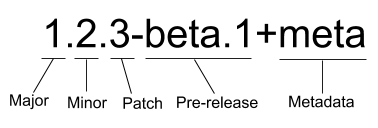
\includegraphics[scale=0.55]{semver}
  \caption{Diagrama de una version en versionamiento semántico.}
  \label{fig:semver}
\end{figure}

Considere la Figura \ref{fig:semver}. Si la versión sólo arregla errores de la versión anterior o alguna previa, entonces
la nueva versión debe ser la misma que la inmediatamente anterior, pero aumentando en una unidad el término \textit{patch}.

Si la versión introduce nuevas funcionalidades, entonces el identificador de la nueva versión debe ser el mimso que la
inmediatamente anterior, pero aumentando en una unidad el término \texttt{minor}.

Finalmente, si la versión introduce un cambio que no es retro-compatible que la versión anterior, entonces se aumenta en una
unidad el término \texttt{major}. Esto ocurre pocas veces, y generalmente implica cambios a nivel estructural del proyecto,
ya sea en su \textit{API}, en su \textit{stack} de tecnologías o algún cambio de requerimientos severo.
Los términos \textit{pre-release} y \textit{metadata} son tan poco utilizados que pueden ser omitidos para efectos de esta memoria.

La primera entrega del proyecto siempre debe ser \texttt{0.1.0}.

Una vez que la entrega ha sido defini, implementada y testeada, están todas las condiciones para hacer la entrega.
La entrega se completa cuando el código ha sido desplegado al ambiente \textit{beta} y se ha notificado al cliente. 

El ambiente \textit{beta} es un ambiente de pre-producción: todas sus configuraciones son como las del ambiente de 
\textit{production}, pero la interacción es sólo con el cliente y algunos usuarios especiales externos (generalmente
otros \textit{stakeholders}). El ambiente de \textit{production} por otro lado, es en dónde los usuarios finales interactúan con la
plataforma.

Al momento de la entrega pueden suceder dos escenarios: si la funcionalidad ejecuta fielmente los requerimientos y el cliente no tiene observaciones
de ningún tipo, entonces el código de la versión se despliega al ambiente de \textit{production} y se finaliza el \textit{sprint}.
Si la funcionalidad falla debido a casos que no se contemplaron, o existen observaciones de requerimientos por parte del cliente,
entonces la versión se extiende al \textit{sprint} siguiente, donde volverá a pasar por los ciclos de Desarrollo y Entrega nuevamente.


\subsection{Post-servicio}
Esta etapa es la última en el ciclo de vida del proyecto e involucra procesos para clientes que terminan la relación
laboral con Nursoft como para aquellos que desean continuarla.

En el caso de los primeros, el código fuente e instrucciones para replicar el despliegue de la plataforma tal cual lo hacía Nursoft
son entregadas al cliente.

En el caso de los segundos, aparece el concepto de plan de mantención para proyectos. 
Este plan se desarrolla en conjunto del área comercial y del área de operaciones y se divide en tres:

\begin{itemize}
  \item \textbf{Infraestructura} Se aloja y administra la plataforma u aplicación desde las cuentas de Nursoft.
  \item \textbf{Garantía} Se realiza mantención correctiva ante desperfectos.
  \item \textbf{Mejora continua} Se desarrollan pequeñas funcionalidades y mejoras.
\end{itemize}

A diferencia del macroproceso principal, esta fase replica la fase de desarrollo de manera muy acotada. Por ejemplo la toma de
requerimientos nuevos o mejoras se acuerda por un hito informal como una llamada telefónica.

Este proceso tambíen busca potenciar el concepto de experiencia para el cliente, y ha ido cambiando en el tiempo en relación
al feedback de los clientes.


% \begin{itemize}
%   \item creación y estandarización de macro-procesos
%   \item Ampliar la cartera de grandes clientes 
% \end{itemize}


% ¿Por qué son relevantes estos puntos? El primero se adhiere lógicamente a lo que esta memoria planea
% establecer: facilitar y alentar la práctica de registrar esfuerzos, mediante una plataforma especializada,
% de la manera más eficiente pero también más lo fiel a la realidad. 
% Este proceso es parte de los macro-procesos de Gestión y de Desarrollo. 

% TODO: Incluir diagramas de Gestión y Desarrollo

% La relevancia del segundo punto no es inmediatamente aparente, por lo que se necesita un poco de contexto.

% Desde 2013 hasta antes de la implementación de esta memoria, Nursoft llevaba la gestión básica de sus
% proyectos utilizando la plataforma Taiga.
% Sus funcionalidades acotadas y simples hicieron un calce perfecto con el Nursoft de ese entonces,
% con proyectos de menor escala, y sin muchos procesos formalizados en la parte de gestión. 
% Taiga utiliza un lenguaje y una interfaz muy cómoda para desarrolladores y jefes de proyecto,
% pero no para \textit{stakeholders} no-técnicos, como clientes y sus asesores.

% Adicionalmente, Taiga es una herramienta muy de nicho. De hecho, según Datanyze, su porcentaje de 
% porción de mercado es bajísimo, como se muestra en la siguiente tabla:

% TODO agregar tabla de Datanyze

% ¿Qué tiene de relevancia este dato? Nursoft ha descubierto en base a clientes de grandes empresas
% con los que trabajó anteriormente, el uso extendido de la plataforma Jira, coincidentemente la plataforma
% que mayor cuota de mercado posee.

% A mediados de año, Nursoft toma la decisión de cambiar de herramienta de gestión de proyecto a Jira,
% pensando en los beneficios de conexión directa con las plataformas de los clientes (si es que las tienen)
% https://www.datanyze.com/market-share/project-management/Alexa%20top%201K?page=10

% \subsection{Reporte}
% Donde se define la estructura de un esfuerzo, en términos de modelado de dato y se contextualiza las partes que componen a un esfuerzo.

% \subsection{Herramientas de gestión de proyecto utilizadas}

% \textit{Donde se explican brevemente las herramientas externas que se utilizan para llevar
% la gestión del proyecto, en términos de historia de usuario, sprints, versiones, etc, y cómo se conectan con la plataforma de reportes}


% \paragraph{Taiga} es un gestor de proyectos \textit{open-source}, con un set de funcionalidades
% enfocadas en la simpleza y creado para startups, desarrollos ágiles y diseñadores.
% Taiga fue liberado en Octubre de 2014 y la última versión fue publicada en Febrero del 2018.

% Utiliza \verb|Django| y \verb|Angularjs| para su backend y su frontend, respectivamente.
% Cuenta con pocas integraciones \textit{out-of-the-box}, pero soporta
% \textit{webhooks}\footnotemark[7] nativamente y cuenta con una API para desarrollar 
% integraciones\cite{taiga_webhooks}\cite{taiga_api}.

% TODO: Mostrar un proyecto en la plataforma Taiga

% \footnotetext[7]{es una estrategia para que dos aplicaciones diferentes se comuniquen, reactivamente, en tiempo real.}

% \paragraph{Jira Cloud} es una herramienta propietaria y pagada de gestión de proyectos. 
% Puede ser utilizada online o ser descargada e instalada localmente, y fue creada
% por la corporación australiana Atlassian. Permite la gestión de proyectos en múltiples metodologías
% ágiles como SCRUM, Kanban, e incluso la gestión de proyectos de otras categorías, como post-venta y
% solución de errores. 

% Es altamente customizable y cuenta con más de 3000 integraciones
% externas \cite{jira_features}. Adicionalmente, cuenta con una API para desarrollar integraciones
% personalizadas \cite{jira_api}.

% TODO: Mostrar un proyecto en la plataforma Jira